%----------
%	CONFIGURACIÓN DEL DOCUMENTO
%----------
\documentclass[12pt]{report} %fuente a 12pt
% MÁRGENES: 2,5 cm sup. e inf.; 3 cm izdo. y dcho.
\usepackage[
  a4paper,
  vmargin=2.5cm,
  hmargin=3cm
]{geometry}

% INTERLINEADO: Estrecho (6 ptos./interlineado 1,15) o Moderado (6 ptos./interlineado 1,5)
\renewcommand{\baselinestretch}{1.15}
\parskip=6pt

% DEFINICIÓN DE COLORES para portada y listados de código
\usepackage[table]{xcolor}
\definecolor{azulUC3M}{RGB}{0,0,102}
\definecolor{gray97}{gray}{.97}
\definecolor{gray75}{gray}{.75}
\definecolor{gray45}{gray}{.45}

\usepackage[a-1b]{pdfx}
\usepackage{hyperref}

\hypersetup{colorlinks=true,
	linkcolor=black, % enlaces a partes del documento (p.e. índice) en color negro
	urlcolor=blue} % enlaces a recursos fuera del documento en azul

% EXPRESIONES MATEMATICAS
\usepackage{amsmath,amssymb,amsfonts,amsthm}

\usepackage{txfonts}
\usepackage[T1]{fontenc}
\usepackage[utf8]{inputenc}

\usepackage[spanish, es-tabla]{babel}
\usepackage[babel, spanish=spanish]{csquotes}
\AtBeginEnvironment{quote}{\small}

% diseño de PIE DE PÁGINA
\usepackage{fancyhdr}
\pagestyle{fancy}
\fancyhf{}
\renewcommand{\headrulewidth}{0pt}
\rfoot{\thepage}
\fancypagestyle{plain}{\pagestyle{fancy}}

% DISEÑO DE LOS TÍTULOS de las partes del trabajo (capítulos y epígrafes o subcapítulos)
\usepackage{titlesec}
\usepackage{titletoc}
\titleformat{\chapter}[block]
{\large\bfseries\filcenter}
{\thechapter.}
{5pt}
{\MakeUppercase}
{}
\titlespacing{\chapter}{0pt}{0pt}{*3}
\titlecontents{chapter}
[0pt]
{}
{\contentsmargin{0pt}\thecontentslabel.\enspace\uppercase}
{\contentsmargin{0pt}\uppercase}
{\titlerule*[.7pc]{.}\contentspage}

\titleformat{\section}
{\bfseries}
{\thesection.}
{5pt}
{}
\titlecontents{section}
[5pt]
{}
{\contentsmargin{0pt}\thecontentslabel.\enspace}
{\contentsmargin{0pt}}
{\titlerule*[.7pc]{.}\contentspage}

\titleformat{\subsection}
{\normalsize\bfseries}
{\thesubsection.}
{5pt}
{}
\titlecontents{subsection}
[10pt]
{}
{\contentsmargin{0pt}
	\thecontentslabel.\enspace}
{\contentsmargin{0pt}}
{\titlerule*[.7pc]{.}\contentspage}

\usepackage{multirow} % permite combinar celdas
\usepackage{caption} % para personalizar el título de tablas y figuras
\usepackage{floatrow} % utilizamos este paquete y sus macros \ttabbox y \ffigbox para alinear los nombres de tablas y figuras de acuerdo con el estilo definido. Para su uso ver archivo de ejemplo
\usepackage{array} % con este paquete podemos definir en la siguiente línea un nuevo tipo de columna para tablas: ancho personalizado y contenido centrado
\newcolumntype{P}[1]{>{\centering\arraybackslash}p{#1}}
\DeclareCaptionFormat{upper}{#1#2\uppercase{#3}\par}

% Diseño de tabla para ingeniería
\captionsetup[table]{
	format=upper,
	name=TABLA,
	justification=centering,
	labelsep=period,
	width=.75\linewidth,
	labelfont=small,
	font=small,
}

\usepackage{graphicx}
\graphicspath{{imagenes/}} %ruta a la carpeta de imágenes

% Diseño de figuras para ingeniería
\captionsetup[figure]{
	format=hang,
	name=Fig.,
	singlelinecheck=off,
	labelsep=period,
	labelfont=small,
	font=small
}

% NOTAS A PIE DE PÁGINA
\usepackage{chngcntr} %para numeración contínua de las notas al pie
\counterwithout{footnote}{chapter}

% LISTADOS DE CÓDIGO
% soporte y estilo para listados de código. Más información en https://es.wikibooks.org/wiki/Manual_de_LaTeX/Listados_de_código/Listados_con_listings
\usepackage{listings}

% definimos un estilo de listings
\lstdefinestyle{estilo}{ frame=Ltb,
	framerule=0pt,
	aboveskip=0.5cm,
	framextopmargin=3pt,
	framexbottommargin=3pt,
	framexleftmargin=0.4cm,
	framesep=0pt,
	rulesep=.4pt,
	backgroundcolor=\color{gray97},
	rulesepcolor=\color{black},
	%
	basicstyle=\ttfamily\footnotesize,
	keywordstyle=\bfseries,
	stringstyle=\ttfamily,
	showstringspaces = false,
	commentstyle=\color{gray45},
	%
	numbers=left,
	numbersep=15pt,
	numberstyle=\tiny,
	numberfirstline = false,
	breaklines=true,
	xleftmargin=\parindent
}

\captionsetup[lstlisting]{font=small, labelsep=period}
% fijamos el estilo a utilizar
\lstset{style=estilo}
\renewcommand{\lstlistingname}{\uppercase{Código}}


\usepackage[backend=biber, style=ieee, isbn=false,sortcites, maxbibnames=5, minbibnames=1]{biblatex} 

% Añadimos las siguientes indicaciones para mejorar la adaptación de los estilos en español
\DefineBibliographyStrings{spanish}{%
	andothers = {et\addabbrvspace al\adddot}
}
\DefineBibliographyStrings{spanish}{
	url = {\adddot\space[En línea]\adddot\space Disponible en:}
}
\DefineBibliographyStrings{spanish}{
	urlseen = {Acceso:}
}
\DefineBibliographyStrings{spanish}{
	pages = {pp\adddot},
	page = {p.\adddot}
}

\addbibresource{./bibliografia/CAAPP.bib} % llama al archivo bibliografia.bib en el que debería estar la bibliografía utilizada



%-------------
%	DOCUMENTO
%-------------

\begin{document}
\pagenumbering{roman} % Se utilizan cifras romanas en la numeración de las páginas previas al cuerpo del trabajo

%----------
%	PORTADA
%----------
\begin{titlepage}
	\begin{sffamily}
	\color{azulUC3M}
	\begin{center}
		\begin{figure}[H] %incluimos el logotipo de la Universidad
			\makebox[\textwidth][c]{
\includegraphics[width=16cm]{Portada_Logo.png}}
		\end{figure}
		\vspace{2.5cm}
		\begin{Large}
			Máster en Ingeniería Informática\\
			2020 - 2021\\
			\vspace{2cm}
			\textsl{Computación de Altas Prestaciones}
			\bigskip

		\end{Large}
		 	{\Huge ``Paralelización de código con OpenMP + MPI''}\\
		 	\vspace*{0.5cm}
	 		\rule{10.5cm}{0.1mm}\\
			\vspace*{0.9cm}
			{\LARGE Carlos Vigil González}\\
            {\LARGE David Gil López}\\
			{\LARGE Daniel Alejandro Rodríguez López}\\
			\vspace*{1cm}
	\end{center}
	\vfill
	\color{black}
	% 
\includegraphics[width=4.2cm]{imagenes/creativecommons.png}\\ %incluimos el logotipo de creativecommons
	% \emph{[Incluir en el caso del interés en su publicación en el archivo abierto]}\\  % BORRAR ESTA LÍNEA
	% Esta obra se encuentra sujeta a la licencia Creative Commons \textbf{Reconocimiento - No Comercial - Sin Obra Derivada}
	\end{sffamily}
\end{titlepage}

%--
% Índice general
%-
\tableofcontents
\thispagestyle{fancy}

%--
% Índice de figuras. Si no se incluyen, comenta las líneas siguientes
%-
\listoffigures
\thispagestyle{fancy}

%--
% Índice de tablas. Si no se incluyen, comenta las líneas siguientes
%-
\listoftables
\thispagestyle{fancy}

%----------
%	TRABAJO
%----------
\clearpage
\pagenumbering{arabic} % numeración con múmeros arábigos para el resto de la publicación

\chapter{Introducción}
\label{chap:Intro}

La presente memoria explica los pasos seguidos, experimentacón y resultados obtenidos durante la
paralelización del código de equalización de histograma entregado inicialmente. Pero antes de entrar
en resultados, conviene explicar en qué consiste una equalización de histograma.

De forma simplista, una equalización de histograma consiste en estirar el rango de valores en una
imagen para aplanar su histograma de valores.

\begin{figure}[H]
    \makebox[\textwidth][c]{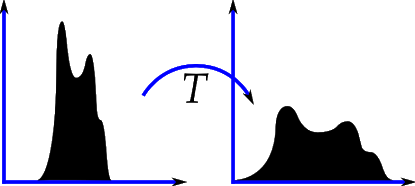
\includegraphics[width=12cm]{histogram_equalization.png}}
    \caption{Ejemplo de Equalización de Histograma}
    \label{fig:hist_eq}
\end{figure}

De forma un poco más técnica, una equalización de histograma distribuye los valores de color en una imagen de forma que todos se encuentran presentes de forma equitativa dentro de la imagen, como se puede apreciar en la \autoref{fig:hist_eq}

Para calcular estos histogramas se debe recorrer la imagen multiples veces, tanto para
calcular los valores iniciales como para establecer los valores finales, por lo tanto hemos orientado
nuestros esfuerzos con OpenMP \parencite{timlewis_openmp_nodate} en optimizar estas iteraciones sobre
la imagen, mientras que con MPI \parencite{noauthor_open_nodate} nos hemos centrado en el reparto
de fragmentos de la imagen entre distintos procesos para reducir el número de iteraciones.

No obstante para poder obtener un análisis más completo de las distintas alternativas y \textit{speed-ups}
posibles, se han realizado 3 versiones distintas de paralelización: \nameref{chap:OpenMP}, \nameref{chap:MPI}
y \nameref{chap:OpenMP+MPI}. De igual forma, para poder comparar los resultados de forma fiable, se ha
utilizado las mismas imágenes de prueba, entorno de ejecución (guernika) y número de ejecuciones.


\subsection{OpenMP}


\subsection{MPI}

En el caso de MPI...


\subsection{Speed up teóricos}

Antes de empezar a realizar ningún cambio sobre el código, con el objetivo de conocer qué mejoras
podemos esperar a la hora de paralelizarlo, se ha calculado un \textit{speed up} teórico para
la \nameref{sec:Amdahl} y para la \nameref{sec:Gustafson}.

\subsubsection{Ley de Amdahl}
\label{sec:Amdahl}

La Ley de Amdahl nos permite dado un programa con carga fija, el \textit{speed up} máximo que podríamos alcanzar

\[ S = \frac{1}{(1 - P) + \frac{P}{N}} \]

Siendo S el \textit{speed up}, P la fracción paralela de código y N el número de núcleos entre
los que la dividimos.

%total = 19+7+59+17+116+70
%paralelo = 7+17+70
De esta forma, en el código original tenemos 288 líneas de código, de las cuales hemos identificado
94 como parelizables, dándo lugar a una $P = 0.32638$.

\begin{figure}[H]
    \makebox[\textwidth][c]{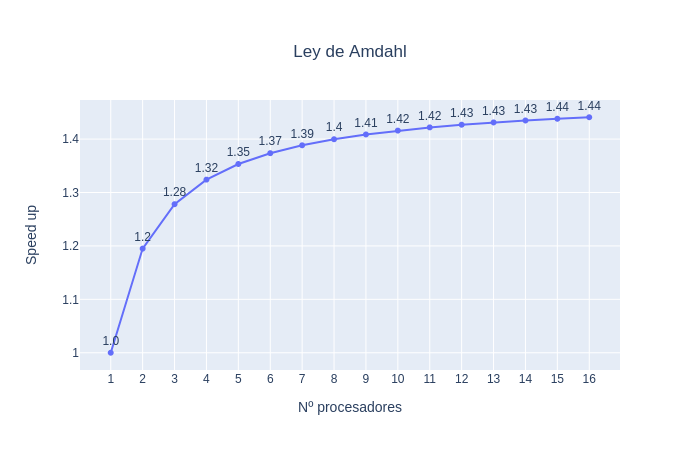
\includegraphics[width=14cm]{amdahl.png}}
    \caption{Ley de Amdahl con distinto N}
    \label{fig:fig_amdahl}
\end{figure}

Como se puede observar el \textit{speed up} se empieza a detener a partir de los 8 procesadores, ya que
de un \textit{speed up} de 1.4 pasamos a 1.44 con 16 procesadores, por lo que no tiene mucho sentido
aumentar el número de procesadores ya que la ganancia sería mínima.

\subsubsection{Ley de Gustafson}
\label{sec:Gustafson}

\[ S = P - \alpha \cdot (P - 1)\]

Siendo P el número de procesadores y $\alpha$ la parte de código no paralelizable.


\chapter{Análisis y experimentación}

En esta sección se describe el análisis de código realizado para determinar qué partes se van a
paralelizar mediante OpenMP y cuales con MPI. También se comentarán las razones por las cuales se ha optado
por elegir cada método en cada caso.

\section{Análisis}

LO DEL VALGRIND

\section{OpenMP}
\label{sec:OpenMP}

La paralelización de código se ha centrado en bucles \textit{for} que operan sobre la imagen,
dado que con OpenMP es muy sencillo seguir un modelo SIMD (\textit{Single Instruction / Multiple Data})
y, además representan un mayor número de iteraciones que cualquier otro tipo de bucles dado que una
imagen pequeña de 200x200 píxeles, se traduciría en 40000 iteraciones.

Empezando por el fichero principal, \textit{contrast.cpp} se han paralelizados los bucles
\textit{for} que se ejecutan a la hora de realizar las lecturas y escrituras de las imágenes de
tipo \textit{PPM}, ya que se itera sobre los tres canales RGB por separado.

En el fichero \textit{contrast-enhancement.cpp} se han paralelizado los bucles que
se encuentran dentro de las funciones que cambian los formatos de color de las imágenes: de \textit{rgb}
a \textit{hsl}, de \textit{hsl} a \textit{rgb}, de \textit{rgb} a \textit{yuv} y de \textit{yuv}
a \textit{rgb}.

En el tercer fichero, \textit{histogram-equalization.cpp}, también se ha realizado la paralelización
de ciertos bucles. Los dos primeros, que se encuentran en la función \textit{histogram}, se ha decidido
optar por paralelizarlos como \textit{SIMD} en vez de como simples bucles for, ya que al tener pocas
iteraciones, el particionarlos no ofrecería ninguna ventaja, pero por otro lado el utilizar las operaciones
vectoriales nos aportaría la velocidad suficiente para contrarestar el \textit{overhead} de paralelizarlo.

Por otro lado, en este mismo fichero también se ha paralelizado el bucle \textit{for} que escribe la imagen
final tras ecualizar el histograma, en este caso usando las directivas propias de los bucles \textit{for} y
de las instrucciones de tipo \textit{SIMD}. El bucle que ecualiza el histograma no ha sido paralelizado
debido a las dependencias que tienen entre una iteración y la anterior.

\subsection{Experimentación}

La experimentación se ha realizado usando la imagen proporcionada de ejemplo (11472 x 6429 píxeles),
usando el entorno de guernika (6 núcleos físicos y otros 6 virtuales, 12 en total a 3,4GHz), variando
el números de hilos usados (desde 1 hasta 16) y repitiendo cada ejecución 100.

En los resultados se pueden observar el tiempo medio obtenido con el código original (para 100 ejecuciones)
y los tiempos medios obtenidos para cada número de hilos de esta versión. 

Partiendo de un valor promedio de ejecuciones secuenciales que se situa en valores cercanos a 0.092 s en grises
y 3.2s en color, diviendo a su ver esto en 0.63s cuando se procesa en formato yuv y 2.48 s cuando se procesa
en hsl. Los valores promedio de la paralelización del codigo son los siguientes:

\begin{figure}[H]
    \makebox[\textwidth][c]{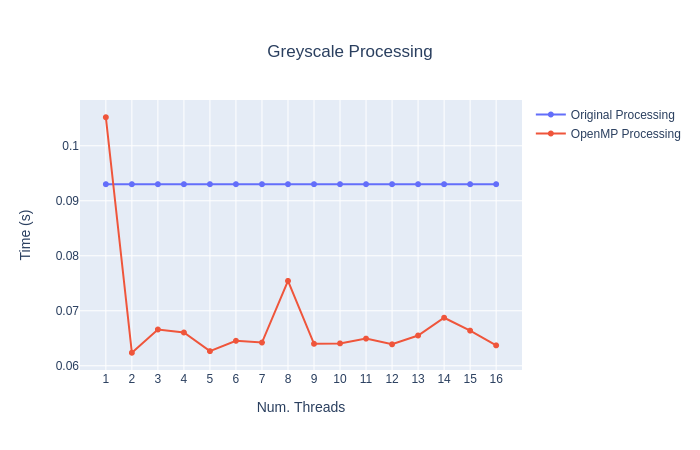
\includegraphics[width=14cm]{omp_grey.png}}
    \caption{Tiempos paralelos sobre tiempo secuencial con OMP}
    \label{fig:fig_omp_grey}
\end{figure}

En esta figura se puede ver que el tiempo empieza siendo peor que en la ejecución secuencial

\section{MPI}
\label{sec:MPI}

La paralelización de código se ha centrado en repartir la carga de trabajo inicial entre los distintos
procesos existentes. De forma similar a OpenMP, la parelización de MPI, aunque puede seguir otros
patrones como MISD (\textit{Multiple Instruction / Single Data}) o MIMD (\textit{Multiple Instruction
/ Multiple Data}), se ha seguido un planteamiento SIMD.

Para decidir en qué secciones del código se puede paralelizar siguiendo un modelo SIMD, hay que identificar
las operaciones que dependen de la imagen completa, para evitar realizar esas operaciones con fragmentos de
la imagen total, ya que se obtendrían resultados distintos de la versión secuencial y por tanto, incorrectos.

Estas secciones de código que dependen de la imagen original se encuentran en la lectura inicial y escritura
final de la misma e inicialización de variables en \textit{contrast.cpp}, en la definición del histograma
inicial y en la normalización del histograma final en \textit{histogram-equalization.cpp}. Sin embargo,
a pesar de depender de la imagen inicial, la inicialización del histograma es fácilmente paralelizable sin
un impacto negativo en el rendimiento al tratarse de un array de números.


\subsection{Experimentación}

La experimentación se ha realizado usando la imagen proporcionada de ejemplo (11472 x 6429 píxeles),
usando el entorno de guernika (6 núcleos físicos y otros 6 virtuales, 12 en total a 3,4GHz), variando
el números de procesos usados (desde 1 hasta 8) y repitiendo cada ejecución 100. El número máximo
de procesos viene limitado por el hardware de la máquina.

En los resultados se pueden observar el tiempo medio obtenido con el código original (para 100 ejecuciones)
y los tiempos medios obtenidos para cada número de procesos de esta versión.

\section{OpenMP + MPI}
\label{sec:OpenMP+MPI}
Explicar "conclusiones" o yuqse sobre porqué en base a lo anterior hemos decidido hacer el OpenMP+MPI final, quizás no es exáctamente igual que simplemente juntar lo anterior


\subsection{Experimentación}

La experimentación se ha realizado usando la imagen proporcionada de ejemplo (11472 x 6429 píxeles),
usando el entorno de guernika (6 núcleos físicos y otros 6 virtuales, 12 en total a 3,4GHz), escogiendo
combinaciones de los mejores parámetros para cada una de las versiones anteriores y repitiendo
durante 100 ejecuciones.

En los resultados se pueden observar el tiempo medio obtenido con el código original (para 100 ejecuciones)
y el tiempo medio obtenido para distintas configuraciones de esta versión.

\chapter{Conclusiones}

Buah colega, hemos aprendido tope mazo



%----------
%	BIBLIOGRAFÍA
%----------

\nocite{*} % Si quieres que aparezcan en la bibliografía todos los documentos que la componen (también los que no estén citados en el texto) descomenta está lína

\clearpage
\addcontentsline{toc}{chapter}{Bibliografía}
\setquotestyle{english} % Cambiamos el tipo de cita porque en el estilo IEEE se usan las comillas inglesas.
\printbibliography


\end{document}
